\chapter[A Parameter Space Exploration of Dust Formation]{A Parameter Space Exploration of Dust Formation within WCd Systems Using an Advected Scalar Dust Model}


\begin{abstract}
    
\end{abstract}

\section{Introduction}

Binary systems with colliding stellar winds are a fascinating phenomena capable of producing a variety of phenomena.
The shocks produced from these interacting systems create some of the most luminous persistent stellar-mass X-ray sources in the night sky \parencite{usov_stellar_1991}.
Within the wind collision region the available mechanical energy rivals the radiative energy of many stars, producing shocks with temperatures up to $10^8$ \si{\kelvin}.

Despite this, in particularly energetic Colliding Wind Binary (CWB) systems, such as those with an evolved Wolf-Rayet (in particular the WC sub-type) star as the source of the dominant wind in the system (A WR+OB binary), dust has been observed to form.
\textcite{allenInfraredPhotometryNorthern1972} first attributed IR excess around WC systems to dust in the form of amorphous carbon grains; however, the high wind temperatures and extremely high luminosities around WC systems are such that dust grains would be readily destroyed through sublimation processes.
Despite this, dust has been observed to form readily in binary systems ( a WCd system), despite an additional highly luminous star and shocks that would quickly destroy dust acting upon these nascent, fragile dust grains.
The exact mechanisms of dust formation as well as the evolution of dust within these systems is poorly understood.
However dust formation rates can be extremely high, up to $10^{-8}$ \si{\solarmass\per\year}, or approximately $0.1\%$ of the total wind by mass.

% Persistent and episodic dust forming systems
% Discuss leading theories briefly

Within different colliding wind binary systems, Dust may form either continuously or periodically.
Whilst the exact mechanism for this condition is not currently known, there is a strong correlation between periodicity and eccentricity, with less eccentric systems forming dust continuously, while highly elliptic systems exhibit periodic dust formation.
Due to this orbital dependency, it is likely that there is an optimal dust forming separation, where dust can form in large quantities. This could be due to factors such as strong post shock cooling, which is highly dependent on the wind speed and orbital separation.
Additionally, dust may be protected from the bulk of the stellar radiation due to the extremely large degree of extinction from the dense post-shock environment.

% Why is it so hard to observe these systems?

Direct observation of dust forming CWBs and in particular the Wind Collision Region (WCR) is exceptionally difficult for a number of reasons:

\begin{itemize}
  \item WR+OB CWB systems are extremely rare, of the 667 catalogued WR stars at time of writing, 106 have been confirmed to be in a binary system \parencite{rossloweSpatialDistributionGalactic2015}.
  \item A WC star is required for dust formation, no Nitrogen sub-type Wolf-Rayet (WN) have been observed to form dust. At time of writing 41 WR binaries contain WC stars.
  \item Not all WC+OB systems are dust producing, limiting the sample size further.
  \item Galactic CWB systems are comparatively distant from earth. For instance, WR 104, a well-studied system, is $\sim 2.5$ \si{\kilo\parsec} distant. This prevents observations of these systems at a high angular resolution.
  \item Based on work by \textcite{zubkoPhysicalModelDust1998a} of CWB systems it appears that grain growth from small nucleation grains is quite rapid, this means that studying the initial grain evolution requires extremely high angular resolution observations.
\end{itemize}

For these reasons, numerical simulations are useful for modelling the growth of dust grains within this unresolved region.
% Proposal of work, what is this project covering?
In order to better understand what influences dust production in a CWB system, a parameter space exploration of the wind and orbital parameters was performed.
In particular the orbital separation, mass-loss rate and wind velocity were modified for both stars in order to influence the wind momentum ratio, $\eta$, and the cooling parameter, $\chi$.
The wind momentum ratio is defined as

\begin{equation}
  \eta = \frac{\dot{\text M}_\text{OB} v^\infty_\text{OB}}{\dot{\text M}_\text{WR}v^\infty_\text{WR}} ,
\end{equation}

\noindent
where $\dot{\text{M}}$ is the mass loss rate of a star and $v^\infty$ is the terminal velocity of a star's outflow.
A low value for $\eta$ indicates that the winds are extremely imbalanced, with one star dominating the wind dynamics of the system.
The wind momentum ratio sets for a given orbital separation, $d_\text{sep}$, the distance from each star to the apex of the wind collision

\begin{subequations}
  \begin{align}
    r_\text{WR} & = \frac{1}{1+\eta^{1/2}} d_\text{sep} , \\
    r_\text{OB} & = \frac{\eta^{1/2}}{1+\eta^{1/2}} d_\text{sep} .
  \end{align}
\end{subequations}

In the case of a very small wind momentum ratio the primary star's wind completely envelopes the secondary stars forming an approximately conical WCR surface.
The half-opening angle of this surface can be estimated by

\begin{equation}
  \theta_c \simeq 2.1 \left( 1 - \frac{\eta^{2/5}}{4}\right) \eta^{-1/3} ~~~ \text{for} ~ 10^{-4} \leq \eta \leq 1 ,
\end{equation}

\noindent
to a high degree of accuracy (\cite{eichler_particle_1993}, but also see \cite{pittardCollidingStellarWinds2018}).
The cooling parameter, $\chi$, compares the cooling time to the escape time from the shock region for a parcel of gas in the immediate post-shock environment. An approximation can be made using the known parameters of a system using the equation:

\begin{equation}
    \chi = \frac{t_\text{cool}}{t_\text{esc}} \approx \frac{v_8^4 d_{12}}{\dot{\text M}_{-7}} , 
\end{equation}

where $v_8$ is the wind terminal velocity in units of $10^8$ \si{cm.s^{-1}}, $d_{12}$ is the distance to the WCR apex in units of $10^{12}$ \si{cm}, and $\dot{\text M}_{-7}$ is the mass loss rate in units of $10^{-7} \si{\solarmass\per\year}$ \parencite{stevens_colliding_1992}.
Small values of $\chi$ indicate that radiative cooling is very important, while $\chi \gg 1$ indicates an adiabatic system.
Strong cooling occurs in comparatively slow, dense winds and is aided by a high metallicity.
As such in many systems the post-shock WR flow will rapidly cool from the immediate post-shock temperature of $10^8 \, \si{\kelvin}$ to temperatures in the dust formation range, $\lesssim 10^4 \, \si{\kelvin}$.
A strongly radiating WCR can be compressed far more as it loses energy.
In comparison, an adiabatic WCR is limited to a maximum density increase of a factor of 4 above the pre-shock wind density. This, combined with the reduction in gas temperature results in rapid dust growth and protection from the stellar UV radiation.

%//TODO Quick section on why this is important

\section{Methodology}

Numerical simulations within this paper utilise the Athena++ hydrodynamical code, a highly modular modern fluid dynamics code \parencite{stoneAthenaAdaptiveMesh2020}.
Simulations are generated in 3D and the Euler hydrodynamical equations are solved in the form:

\begin{subequations}
  \begin{align}
    \frac{\partial\rho}{\partial t}+\nabla \cdot \left(\rho \boldsymbol{u}\right) & = 0 , \\
    \frac{\partial \rho \boldsymbol{u}}{\partial t} + \nabla \cdot \left(\rho \boldsymbol{u} u + P \right) & = 0, \\
    \frac{\partial \rho \varepsilon}{\partial t} + \nabla \cdot \left[ \boldsymbol{u} \left( \rho\varepsilon + P \right) \right] & = \dot E_{cool} , 
  \end{align}
\end{subequations}

\noindent
where $\varepsilon$ is the total specific energy ($\varepsilon = \boldsymbol{u}^2/2 + e/\rho $, $\rho$) is the mass density, $e$ is the internal energy density, $P$ is the gas pressure and $u$ is the gas velocity.
In order to simulate radiative losses, the parameter $\dot E_{cool}$ is included, which is the energy loss rate per unit volume from the fluid due to gas and dust cooling, which is elaborated on in section \ref{sec:gas-dust-cooling}.

% Technical details

Athena++ has been configured to run using a piecewise linear reconstruction method with a 4\ts{th} order Strong Stability Preserving Runge-Kutta time-integration method \parencite{spiteriNewClassOptimal2002}.
Athena++ was forked from the original repository and additional routines were written for a Colliding Wind Binary case.
Routines were created to produce a steady outflow from a small spherical region around a set of cartesian co-ordinates as well as a function to move these co-ordinates with each time-step; these were used to simulate stellar wind outflow and orbital motion, respectively.
Additionally, Athena++ was further modified to include an advected scalar dust model for simulating dust growth and destruction as well as a photon emission cooling model to approximate cooling for gas and dust particles within the fluid.

Athena++ utilises OpenMPI for parallelism, breaking the simulation into blocks, which are distributed between processors.
The block size is variable, but for these simulations a block size of $32\times 32 \times 8$ was found to be optimal.
This meshblock system is also utilised in mesh refinement for increasing effective resolution.
As the CWB systems are being simulated in their entirety, a very large volume needs to be simulated, while at the same time the region between the stars must be resolved with a resolution of at least 100 cells in order to adequately resolve the WCR.
This difference in length scales necessitates the use of static mesh refinement (SMR) to improve the effective resolution of the simulation.
A base coarse resolution of $320 \times 320 \times 40$ cells is defined for the simulations, while a region close to the binary pair operates at a higher refinement level, resulting in a resolution increase with a factor of $2^{n-1}$ greater than the coarse resolution, where $n$ is the refinement level (figure \ref{fig:smr-grid}).
this results in an effective resolution of $20480 \times 20480 \times 2560$ cells.
SMR is utilised instead of Adaptive Mesh Refinement, a more flexible conditional method, as it has proven to be more reliable within Athena++, as it mitigates unintentional over-refinement.
As much of the grain evolution occurs a small distance from the WCR stagnation point, much of the simulation can be run at a lower resolution without affecting the simulation outcome.

\begin{figure}
  \centering
  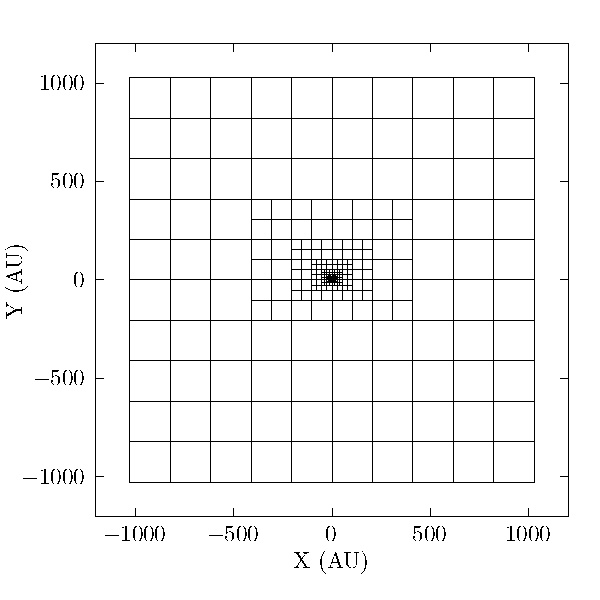
\includegraphics{assets/mesh/gridxy.pdf}
  \caption[Static mesh refinement example]{Plot of blocks used in a 7 level simulation with a block size of $32\times 32 \times 8$ cells. The block density increases dramatically closer to the barycentre.}
  \label{fig:smr-grid}
\end{figure}

The wind outflow from each star is simulated by replacing the conserved variables (density, momentum and energy) within a small region around the expected position of the stars; this region is typically on the order of 6 maximally refined cells in radius.
This rewrite corresponds to a change in mass and mechanical energy imparted by an outflowing wind, such that

\begin{subequations}
  \begin{align}
    \rho_R & = \frac{\dot M}{(4 \pi r^2 v_\infty)} , \\
    p_{R}  & = \rho_R v_\infty , \\
    E_R    & = \frac{P_R}{\gamma - 1} + \frac{1}{2} \rho_{R} v_\infty^2 ,
  \end{align}
\end{subequations}

% This may need more explanation, depending on previous equations
\noindent
where $v_r$ is the wind velocity as it flows radially from the center of the ``remap zone'', $P_R$ is the remap pressure, $P_R = \rho_R k_B T_w / \mu m_H$, $T_w$ is the wind temperature and $r$ is the distance from the current cell to the centre of the remap zone.
Orbits are calculated by moving the remap zones in a manner consistent with Keplerian dynamics, which are updated at every timestep.

% Plasma and dust cooling

\subsection{Gas and dust cooling} \label{sec:gas-dust-cooling}

Cooling due to photon emission from atoms, ions and free electrons, as well as dust particles is simulated by removing energy from a cell at each timestep.
The total energy loss is calculated by integrating the energy loss rates due to gas, plasma and dust cooling using the Euler method; in regions with very rapid cooling sub-stepping is used to improve accuracy, with the number of sub-steps being determined by comparing the substep time to the cooling timescale of the cell.
Gas cooling is simulated using a lookup table method.
A data file containing the gas temperature and associated normalised emissivity, $\Lambda(T)$ of the wind at that temperature is read into the simulation.
In a typical cooling step, the temperature is calculated and a binary search is performed to find the nearest temperature in the lookup table.
A linear interpolation is then performed to find an appropriate value for $\Lambda$.
Energy loss can be calculated with the formulae:

\begin{equation}
  \frac{dE}{dt} = \left(\frac{\rho}{m_H}\right)^2 \Lambda_w(T),
\end{equation}

\noindent
where $\rho$ is the gas density and $m_H$ is the mass of a hydrogen atom.
The lookup table was generated by mixing a series of cooling curves generated by MEKAL simulations of elemental gasses.
These are combined based on the elemental abundances of each wind such that:

\begin{subequations}
  \begin{align}
    \Lambda_\text{WR}(T) & = n_e n_i \sum{X_\text{WR} \Lambda_\text{WR}{E}(T)}, \\
    \Lambda_\text{OB}(T) & = n_e n_i \sum{X_\text{OB} \Lambda_\text{OB}{E}(T)},
  \end{align}
\end{subequations}

\noindent
where $n_e$ and $n_i$ are the electron and ion number density, $X$ is the abundance of an element, and $\Lambda_E(T)$ is the cooling parameter of an element.
Figure \ref{fig:cooling-curve} shows the cooling curves used for each star.
Two lookup tables are used in the simulations, based on the elemental abundances of each star. 
The Wolf-Rayet star uses a curve with abundances typical of a WC9 star with total hydrogen depletion and a high carbon mass fraction, while the OB star is assumed to have solar abundances.
The most significant abundances used in this projects simulations are presented in table \ref{tab:abundances}.
The cooling regime of this code ranges from $10^4$ to $10^9\,\si{\kelvin}$.
A floor temperature of $10^4$ \si{\kelvin} is implemented, temperatures between $\SI{1e4}{\kelvin} < T \leq \SI{1.1e4}{\kelvin}$ are reduced to $10^4\,\si{\kelvin}$ as they are assumed to be either rapidly cooling or a part of the stellar wind.

\begin{table}
  \centering
  \begin{tabular}{@{}ccc@{}}
  \toprule
  \multicolumn{1}{l}{} & \multicolumn{2}{c}{X(E)} \\ \cmidrule(l){2-3} 
   & Solar & WC9 \\ \midrule
  H & $0.705$ & $0.0$ \\
  He & $0.275$ & $0.546$ \\
  C & $3.07 \times 10^{-3}$ & $0.4$ \\
  N & $1.11 \times 10^{-3}$ & $0.0$ \\
  O & $9.60 \times 10^{-3}$ & $0.05$ \\
  % Ne & $1.75 \times 10^{-3}$ & $0.0$ \\
  % Na & $3.47 \times 10^{-5}$ & $3.47 \times 10^{-5}$ \\
  % Mg & $7.10 \times 10^{-4}$ & $7.10 \times 10^{-4}$ \\
  % Al & $6.13 \times 10^{-5}$ & $6.13 \times 10^{-5}$ \\
  % Si & $8.60 \times 10^{-4}$ & $8.60 \times 10^{-4}$ \\
  % S & $3.82 \times 10^{-4}$ & $3.82 \times 10^{-4}$ \\
  % Ar & $1.01 \times 10^{-4}$ & $1.01 \times 10^{-4}$ \\
  % Ca & $6.15 \times 10^{-5}$ & $6.15 \times 10^{-5}$ \\
  % Fe & $1.52 \times 10^{-3}$ & $1.52 \times 10^{-3}$ \\
  % Ni & $7.65 \times 10^{-5}$ & $7.65 \times 10^{-5}$ \\ \bottomrule
  \end{tabular}
  \caption[Abundances used for OB and WR stars]{Abundances used for the OB and WR stars being simulated, other elements are assumed trace when calculating radiative energy loss due to dust.}
  \label{tab:abundances}
\end{table}


\begin{figure}[ht]
  \centering
  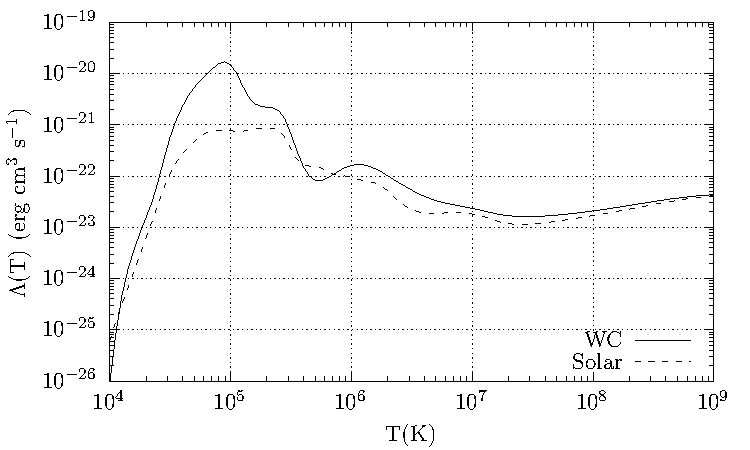
\includegraphics{assets/cooling-curve/cooling-curve-no-elements.pdf}
  \caption[WR and OB $\Lambda(T)$ cooling curves]{Comparison of lookup tables for calculating energy loss due to gas cooling.}
  \label{fig:cooling-curve}
\end{figure}

A model for cooling due to emission from dust grains is also included as dust cooling is expected to play a significant role in the evolution of each system.
The rate of cooling is calculated using the uncharged particle case of the \textcite{dwek_infrared_1981} prescription.
Grains are heated due to collisions with ions and electrons, causing them to radiate, with energy being removed from the simulation.
This assumes that the region being simulated is optically thin to far infrared photons.
The energy loss rate is calculated with the following formulae:

\begin{subequations}
  \begin{align}
    H_\text{coll} & = 1.26 \times 10^{-19} \frac{n}{A^{1/2}} a^2(\mu \text m) T^{3/2} h(a,T) , \\
        \Lambda_d & = \frac{H_\text{coll} + H_\text{el}}{n_H} , \\
    \frac{dE}{dt} & = n_T n_d \Lambda_d ,
  \end{align}
\end{subequations}

\noindent
where $H_\text{coll}$ is the heating rate due to atom and ion collisions, $H_\text{el}$ is the heating rate due to electron collisions, $h(a,T)$ is the grain-ion transparency and $n_T$ is the total ion number density.
$H_\text{coll}$ is summated for Hydrogen, Helium, Carbon, Nitrogen and Oxygen atom collisions.
Other elements are not considered as they are present in trivial proportions in both winds.

\begin{figure}[h]
  \centering
  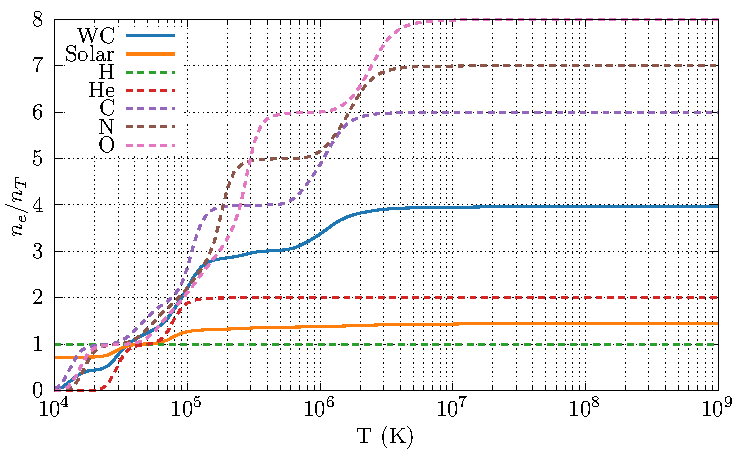
\includegraphics{assets/ionisation-fraction/ionisation-fraction.pdf}
  \caption[OB and WR electron-ion ratios]{A comparison of the electron-ion ratio of both winds as the temperature changes. Included are the pure wind flows that the lookup tables are built from.}
  \label{fig:electron-curve}
\end{figure}

Electron-grain collisions are modelled similarly to ions, albeit with some differences.
One major factor for calculating accurate energy loss due to electron collisions is that the electron number density needs to be accurately calculated; this is performed with a second series of lookup tables that contain the electron-to-ion ratio of each wind across a temperature range of $10^4$ to $10^9\si{\kelvin}$ (figure \ref{fig:electron-curve}).
The electron number density is found to be $n_e = \beta n_i$ where $\beta$ is the electron-to-ion ratio and $n_i$ is the ion number density.
Another difference between calculating electron-grain and gas-grain cooling is calculating electron-grain transparency, which is a significantly more complex problem than calculating ion-grain transparency.
An assumed full opacity proves to be extremely inaccurate at temperatures $>10^6$ \si{\kelvin}.
Electron-grain transparency is therefore calculated via an approximation described in \textcite{dwek_infrared_1981}:

\begin{equation}
  \begin{alignedat}{3}
    h(x^*) & = 1 ,                && ~~ x^* > 4.5, \\
           & = 0.37{x^*}^{0.62} , && ~~ x^* > 1.5 , \\
           & = 0.27{x^*}^{1.50} , && ~~ \text{otherwise,}
  \end{alignedat}
\end{equation}

\noindent
where $x^* = \num{2.71e8} a^{2/3} (\si{\micro\metre})/T$.
This approximation is approximately 4 orders of magnitude faster than using an integration method, while only being out by $\sim 8\%$ in the worst case scenario (figure \ref{fig:lambdacomparison}).
Grain-grain collisions are not modelled, as this would be difficult to calculate due to the single-fluid model in use.
Further simulations utilising a multi-fluid model could allow for this to be simulated.

\begin{figure}
  \centering
  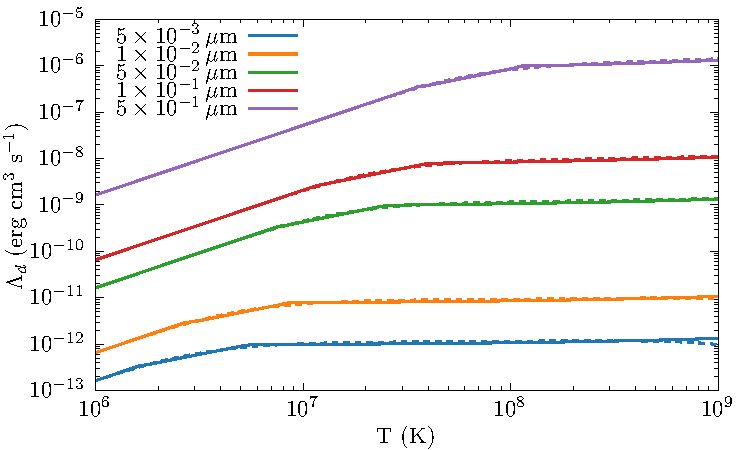
\includegraphics{assets/grain-transparency/lambda-comp.pdf}
  \caption[Comparison of electron transparency methods.]{$\Lambda_d$ as a function of temperature for various grain sizes. The estimate method is extremely close to the integral value aside from at the highest temperatures.}
  \label{fig:lambdacomparison}
\end{figure}

\subsection{Numerical modelling of dust through advected scalars}

The most important modification to Athena++ was the addition of a dust growth and destruction model to simulate the production of dust within the WCR.
A passive scalar model was used where dust can evolve and advect through the simulation, analogous to a co-moving fluid, which previous papers have noted is an accurate dynamical model for dust within the WCR \parencite{hendrix_pinwheels_2016}.
In these simulations, dust is stored in the form of two variables, the average grain radius, $a$, and the dust-to-gas mass ratio, $z$.
From these constants the dust production rate, number density, and total dust mass can be derived.
A co-moving model allows for a simplified model of dust formation. In such a model, the mean particle velocity between two particles of different size can be given as:

\begin{equation}
  \langle u \rangle = \left[ \frac{8kT}{\pi m_r} \right] ^{1/2} ,
\end{equation}

\noindent
where $m_r$ is the familiar reduced mass between a test particle of mass $m_t$ and a field particle of mass $m_f$

\begin{equation}
  m_r = \frac{m_f m_t}{m_f + m_t} .
\end{equation}

\noindent
As the dust grain is significantly more massive, the reduced mass is approximately equal to the grain mass, simplifying the dynamics of the simulation in a co-moving case.
Dust growth is modelled through approximating growth due to grain-gas accretion where grains co-moving with a gas perform relatively low-velocity collisions with the surrounding gas, causing it to accrete onto the surface of the dust grain \parencite{spitzer_jr._physical_2008}.
Assuming a single average grain size the change in average grain radius is given by

\begin{equation}
  \frac{da}{dt} = \frac{\xi_a \rho_{Gr} w_a}{4 \rho} ,
\end{equation}

\noindent
where $w_a$ is the Maxwell-Boltzmann distribution RMS velocity, $\xi_a$ is the grain sticking efficiency and $\rho_{Gr}$ is the grain bulk density.
The associated rate of dust density change is found to be

\begin{equation}
  \frac{d\rho_D}{dt}  = 4 \pi a^2 \rho_g n_D \frac{da}{dt} , 
\end{equation}

\noindent
where $\rho_g$ is the gas density and $n_D$ is the grain number density.
In this paper $\xi_a$ is assumed to be $10\%$ while a bulk density analogous to amorphous carbon grains of $3 \, \si{g.cm^{-3}}$ is utilised.

Dust destruction is calculated via gas-grain sputtering using the \textcite{draine_destruction_1979} prescription - a dust grain has a lifespan, $\tau$, which is dependent on the grain radius.
Assuming a spherical grain, the rate of change in mass and radius can be calculated such that:

\begin{subequations}
  \begin{align}
           \tau_D & = 1 \, \text{Myr} \times \frac{a}{n_g} , \\
    \frac{da}{dt} & = - \frac{a}{\tau_D} , \\
    \frac{dm}{dt} & = -1.33 \times 10^{-13} a^2 n_g n_d \rho_{Gr} ,
  \end{align}
\end{subequations}

\noindent
where $n_g$ is the gas number density.

% //TODO cleanup sentence structures

In order to propagate dust through each simulation, a small initial value for the advected scalars is set in each cell in the remap zones.
A minimum grain radius of $50 \, \text{\AA}$ and minimum dust-to-gas mass ratio of $10^{-6}$ is imposed.
Changing $z_{min}$ does not significantly impact the final dust-to-gas mass ratio of the system as $z$ rapidly increases within the WCR and dust growth in the WCR dominates the total production.

\section{Model Parameters}

In this paper we do not intend on modelling particular systems.
Rather we intend to gain a deeper understanding of what the primary influences of dust formation are in a CWB system.
A series of simulations were therefore run in order to determine how dust formation varies due changes in orbital separation and wind momentum ratio.
A baseline simulation with properties similar to WR98a with a circular orbit and identical stellar masses was created.
Additionally, this baseline simulation has a momentum ratio of $0.02$.
Other simulations were then run with different orbital separations and/or wind momentum ratios.
Another set of simulations were run where the cooling mechanisms were selectively disabled, in order to understand how radiative cooling effects the dust production rate.
Table \ref{tab:baseline-windproperties} and \ref{tab:baseline-orbits} detail the wind and orbital parameters of the baseline simulation.
The orbital separation is modified by changing the orbital period of the simulation, while wind momentum ratio is modified by adjusting the mass loss ratio and wind terminal velocity for each star.
Two simulation sub-sets for this were performed, simulations where the wind terminal velocities were adjusted for each star and simulations where the mass loss rates for each star were adjusted.

\begin{table}
  \centering
  \begin{tabular}{cccc}
  \hline
  Parameter & WR & OB & Unit \\ \hline
  $\dot M$ & \num{5.0e-6} & \num{5.0e-8} & \si{\solarmass\per\year} \\
  $v_\infty$ & \num{1.0e8} & \num{2.0e8} & \si{cm.s^{-1}} \\
  $T_w$ & \num{1.0e4} & \num{1.0e4} & K \\
  \hline
  \end{tabular}
  \caption{Wind properties of the baseline system.}
  \label{tab:baseline-windproperties}
\end{table}

\begin{table}
  \centering
  \begin{tabular}{ccc}
  \hline
  Parameter & Value & Unit \\ \hline
  $M$ & 10.0 & \si{\solarmass} \\
  $d_{sep}$ & \num{4.0} & \si{\au} \\
  $P$ & \num{1.80} & \si{\year} \\
  \hline
  \end{tabular}
  \caption{Baseline system orbital properties.}
  \label{tab:baseline-orbits}
\end{table}

\subsection{Cooling mechanisms}

For this set of simulations, the influence of cooling was changed by varying how cooling works within the simulations.
All simulations in this set keep the same orbital and wind parameters, which are that of the baseline system described in tables \ref{tab:baseline-windproperties} \& \ref{tab:baseline-orbits}.
One simulation has both plasma and dust cooling in operation (the \texttt{fullcool} simulation), while the other two simulations have plasma cooling only and no cooling respectively (\texttt{plasmacool} and \texttt{nocool}, table \ref{tab:cooling-param}).
The final, no radiative cooling simulation instead relies on adiabatic expansion for temperature change; as such, this simulation behaves as if it has a $\chi$ value for both winds that is arbitrarily high.
The post-shock flow in the \texttt{nocool} model will also be unable to compress as much due to the lack of energy loss via radiative cooling.
The role of these simulations is to discern whether it is cooling alone or other system parameters that affects dust production.

% Discuss why this is important, mention overdensity due to radiative cooling

\begin{table}
  \centering
  \begin{tabular}{ccc}
    \hline
    Name & Plasma cooling & Dust cooling \\
    \hline
    \texttt{fullcool} & Yes & Yes \\ 
    \texttt{plasmacool} & Yes & No \\
    \texttt{nocool} & No & No \\
    \hline
  \end{tabular}
  \caption{Cooling series simulation parameters}
  \label{tab:cooling-param}
\end{table}

\subsection{Wind momentum ratio}

Another set of simulations was devised in order to assess the influence of the wind parameters on the formation of dust within a CWB.
As the wind momentum ratio is dependent on both the mass loss rate and wind velocity of each star, each of these properties is modified over a course of simulations.
$\eta$ is varied from 0.01 to 0.04 by adjusting the wind parameters for each star.
This is further subdivided by which property is modified, either the mass loss rate (table \ref{tab:mdot-param}) or wind terminal velocity (table \ref{tab:vinf-param}).
As the cooling parameter has a much stronger dependency on $v_\infty$ than $\dot{\text{M}}$, the modification of either parameter while maintaining a similar value for $\eta$ allows us to determine whether the cooling parameter is the primary characteristic determining the formation of dust within WCd systems.
This can be seen when comparing simulations \texttt{mdot-1} and \texttt{vinf-1}, which have similar wind momentum ratios but the cooling parameters for the WC star differ by a factor of 32.
These simulations are compared to the baseline simulation, which a radiative post-shock WCR.
Whilst the simulations with $\eta = 0.00$ still have very imbalanced winds, they are typical of a WR+OB binary with a less intense Wolf-Rayet partner star wind.
All simulations were run for a minimum of 1 orbit.
As these orbits are circular, there should be no major variance of the winds after the start-up transients are fully advected, save for some fluctuations.

\begin{table}
  \centering
  \begin{tabular}{cccccccc}
  \hline
  Name & $\dot M_{WR}$ & $\dot M_{OB}$ & $v^\infty_{WR}$ & $v^\infty_{OB}$ & $\eta$ & $\chi_{WR}$ & $\chi_{OB}$ \\ 
  & \si{\solarmass\per\year} & \si{\solarmass\per\year} & \si{\centi\metre\per\second} & \si{\centi\metre\per\second} & & & \\ \hline
  \texttt{baseline}& \num{5.0e-6} & \num{5.0e-8} & \num{1e8} & \num{2e8} & 0.02 & 1.20 & 1915 \\
  \texttt{mdot-1}  & \num{1.0e-5} & \num{5.0e-8} & \num{1e8} & \num{2e8} & 0.01 & 0.60 & 1915 \\
  \texttt{mdot-2}  & \num{2.5e-6} & \num{5.0e-8} & \num{1e8} & \num{2e8} & 0.04 & 2.39 & 1915 \\
  \texttt{mdot-3}  & \num{5.0e-6} & \num{1.0e-7} & \num{1e8} & \num{2e8} & 0.04 & 1.20 & 957  \\
  \texttt{mdot-4}  & \num{5.0e-6} & \num{2.5e-8} & \num{1e8} & \num{2e8} & 0.01 & 1.20 & 3830 \\
  \hline
  \end{tabular}
  \caption[Mass loss rate series wind parameters]{Wind parameters for simulations varying the mass loss rate, $\dot M$.}
  \label{tab:mdot-param}
\end{table}

\begin{table}
  \centering
  \begin{tabular}{cccccccc}
  \hline
  Name & $\dot M_{WR}$ & $\dot M_{OB}$ & $v^\infty_{WR}$ & $v^\infty_{OB}$ & $\eta$ & $\chi_{WR}$ & $\chi_{OB}$ \\ 
  & \si{\solarmass\per\year} & \si{\solarmass\per\year} & \si{\centi\metre\per\second} & \si{\centi\metre\per\second} & & & \\ \hline
  \texttt{baseline} & \num{5e-6} & \num{5e-8} & \num{1e8} & \num{2e8} & 0.02 & 1.20 & 1915  \\
  \texttt{vinf-1}   & \num{5e-6} & \num{5e-8} & \num{2e8} & \num{2e8} & 0.01 & 19.1 & 1915  \\
  \texttt{vinf-2}   & \num{5e-6} & \num{5e-8} & \num{5e7} & \num{2e8} & 0.04 & 0.07 & 1915  \\
  \texttt{vinf-3}   & \num{5e-6} & \num{5e-8} & \num{1e8} & \num{4e8} & 0.04 & 1.20 & 30638 \\
  \texttt{vinf-4}   & \num{5e-6} & \num{5e-8} & \num{1e8} & \num{1e8} & 0.01 & 1.20 & 120   \\
  \hline
  \end{tabular}
  \caption[Terminal velocity series wind parameters]{Wind parameters for simulations varying the wind terminal velocity, $v^\infty$.}
  \label{tab:vinf-param}
\end{table}

\subsection{Separation distance}

A final series of simulations was performed with the wind parameters equivalent to the baseline model, but with differing orbital separations.
The separation was altered by modifying the orbital period of each star, as stellar masses were to be kept realistic.
The separation distance was varied from the baseline model of 4 \si{\au} to 64 \si{\au} (table \ref{tab:dsep-param}), which has the effect of modifying the cooling parameter of each simulation without changing the wind momentum ratio; allowing us to further discern which is the dominant parameter influencing dust formation.
For instance, simulation \texttt{dsep-64AU} has a cooling parameter value approaching the fast WR wind model \texttt{vinf-1}, despite having a wind momentum ratio of 0.02.

%//TODO this section needs some analytical work, specifically on the expected values for dt, things like that, I can also get some stuff from the results

Each simulation has a coarse resolution of $320 \times 320 \times 40$ cells, with a varying number of levels, as the separation distance is doubled, the associated static mesh refinement box is halved and the number of levels is decremented. This manipulation of levels ensures that the number of cells between the stars is kept consistent, reduces memory usage and keeps the average timestep approximately the same.
The simulation extent was doubled over the previous simulations, to approximately $2000 \times 2000 \times 250 \, \si{\au}$.
Similarly to the previous set of simulations, a minimum of 1 orbit was needed for each simulation, however, as the orbital period of each simulation varies, certain simulations were able to run for a significantly longer length of time, with data for multiple orbits being obtained.

\begin{table}[h]
  \centering
  \begin{tabular}{ccccccc}
    \hline
    Name & P & $d_{sep}$ & $\chi_{WR}$ & $\chi_{OB}$ & Levels & Effective Resolution \\
    & \si{\year} & \si{\au} & & & & Cells \\ \hline 
    \texttt{dsep-4AU}  & \num{1.80} & 4  & 1.20 & 1915  & 7 & $20480 \times 20480 \times 2560$ \\
    \texttt{dsep-8AU}  & \num{5.06} & 8  & 2.39 & 3830  & 6 & $10240 \times 10240 \times 1280$ \\
    \texttt{dsep-16AU} & \num{14.3} & 16 & 4.79 & 7659  & 5 & $5120 \times 5120 \times 640$    \\
    \texttt{dsep-32AU} & \num{40.5} & 32 & 9.57 & 15319 & 4 & $2560 \times 2560 \times 320$    \\
    \texttt{dsep-64AU} & \num{115}  & 64 & 19.1 & 30638 & 3 & $1280 \times 1280 \times 160$    \\ \hline
  \end{tabular}
  \caption{Parameters of simulations varying separation distance.}
  \label{tab:dsep-param}
\end{table}

\subsection{Data collection}

Data was collected in multiple forms.
HDF5 files were generated at regular time intervals - 3D HDF5 meshes were generated every $1/100^{\text{th}}$ of an orbit, while 2D slices were produced every $1/1000^{th}$ of an orbit.
These HDF5 files contain the primitive variables of the simulation, gas density, $\rho$, gas pressure, $P$ and wind velocity components, $v_x$, $v_y$ and $v_z$; these can be used to derive other variables such as the gas temperature as well as the internal, kinetic and total energies.
The scalars governing the dust properties were also stored for each cell, the dust-to-gas mass ratio, $z$ and the dust grain radius, $a$.
The wind ``colour'' was also tracked.
This is the proportion of gas resultant from each star; a value of 1.0 is a pure WR wind, 0.0 is a pure OB wind, while 0.5 is a perfectly mixed wind.
In addition to HDF5 outputs, the volume-weighted summations of all system parameters, such as the total system mass and summated average grain radius were collected.
In order to derive average values, such as $\bar{z}$ and $\bar{a}$, the values for each can be divided by the total system mass.
To calculate dust formation within the WCR, a method of determining if a cell was a part of the wind collision region was devised - the cell density would be compared to the predicted density of a single smooth wind with the wind parameters of the Wolf-Rayet star in the system:

\begin{equation}
  \rho_\text{SW} = \frac{\dot{M}_{WR}}{4 \pi r^2 v^\infty_{WR}},
\end{equation}

\noindent
where $r$ is the distance from the barycentre. This threshold value was set to $1.25\rho_\text{SW}$ as it most accurately determined if a cell was part of the WCR.
Increased threshold values were not accurate at large distances from the barycentre (figure \ref{fig:overdensity-threshold}).
Other methods of detecting the Wind Collision Region such as determining wind mixing levels were not successful in general.
A mixed wind model for detecting over-density was also considered, however it was not any more accurate than the single wind over-density model. 

\begin{figure}
  \centering
  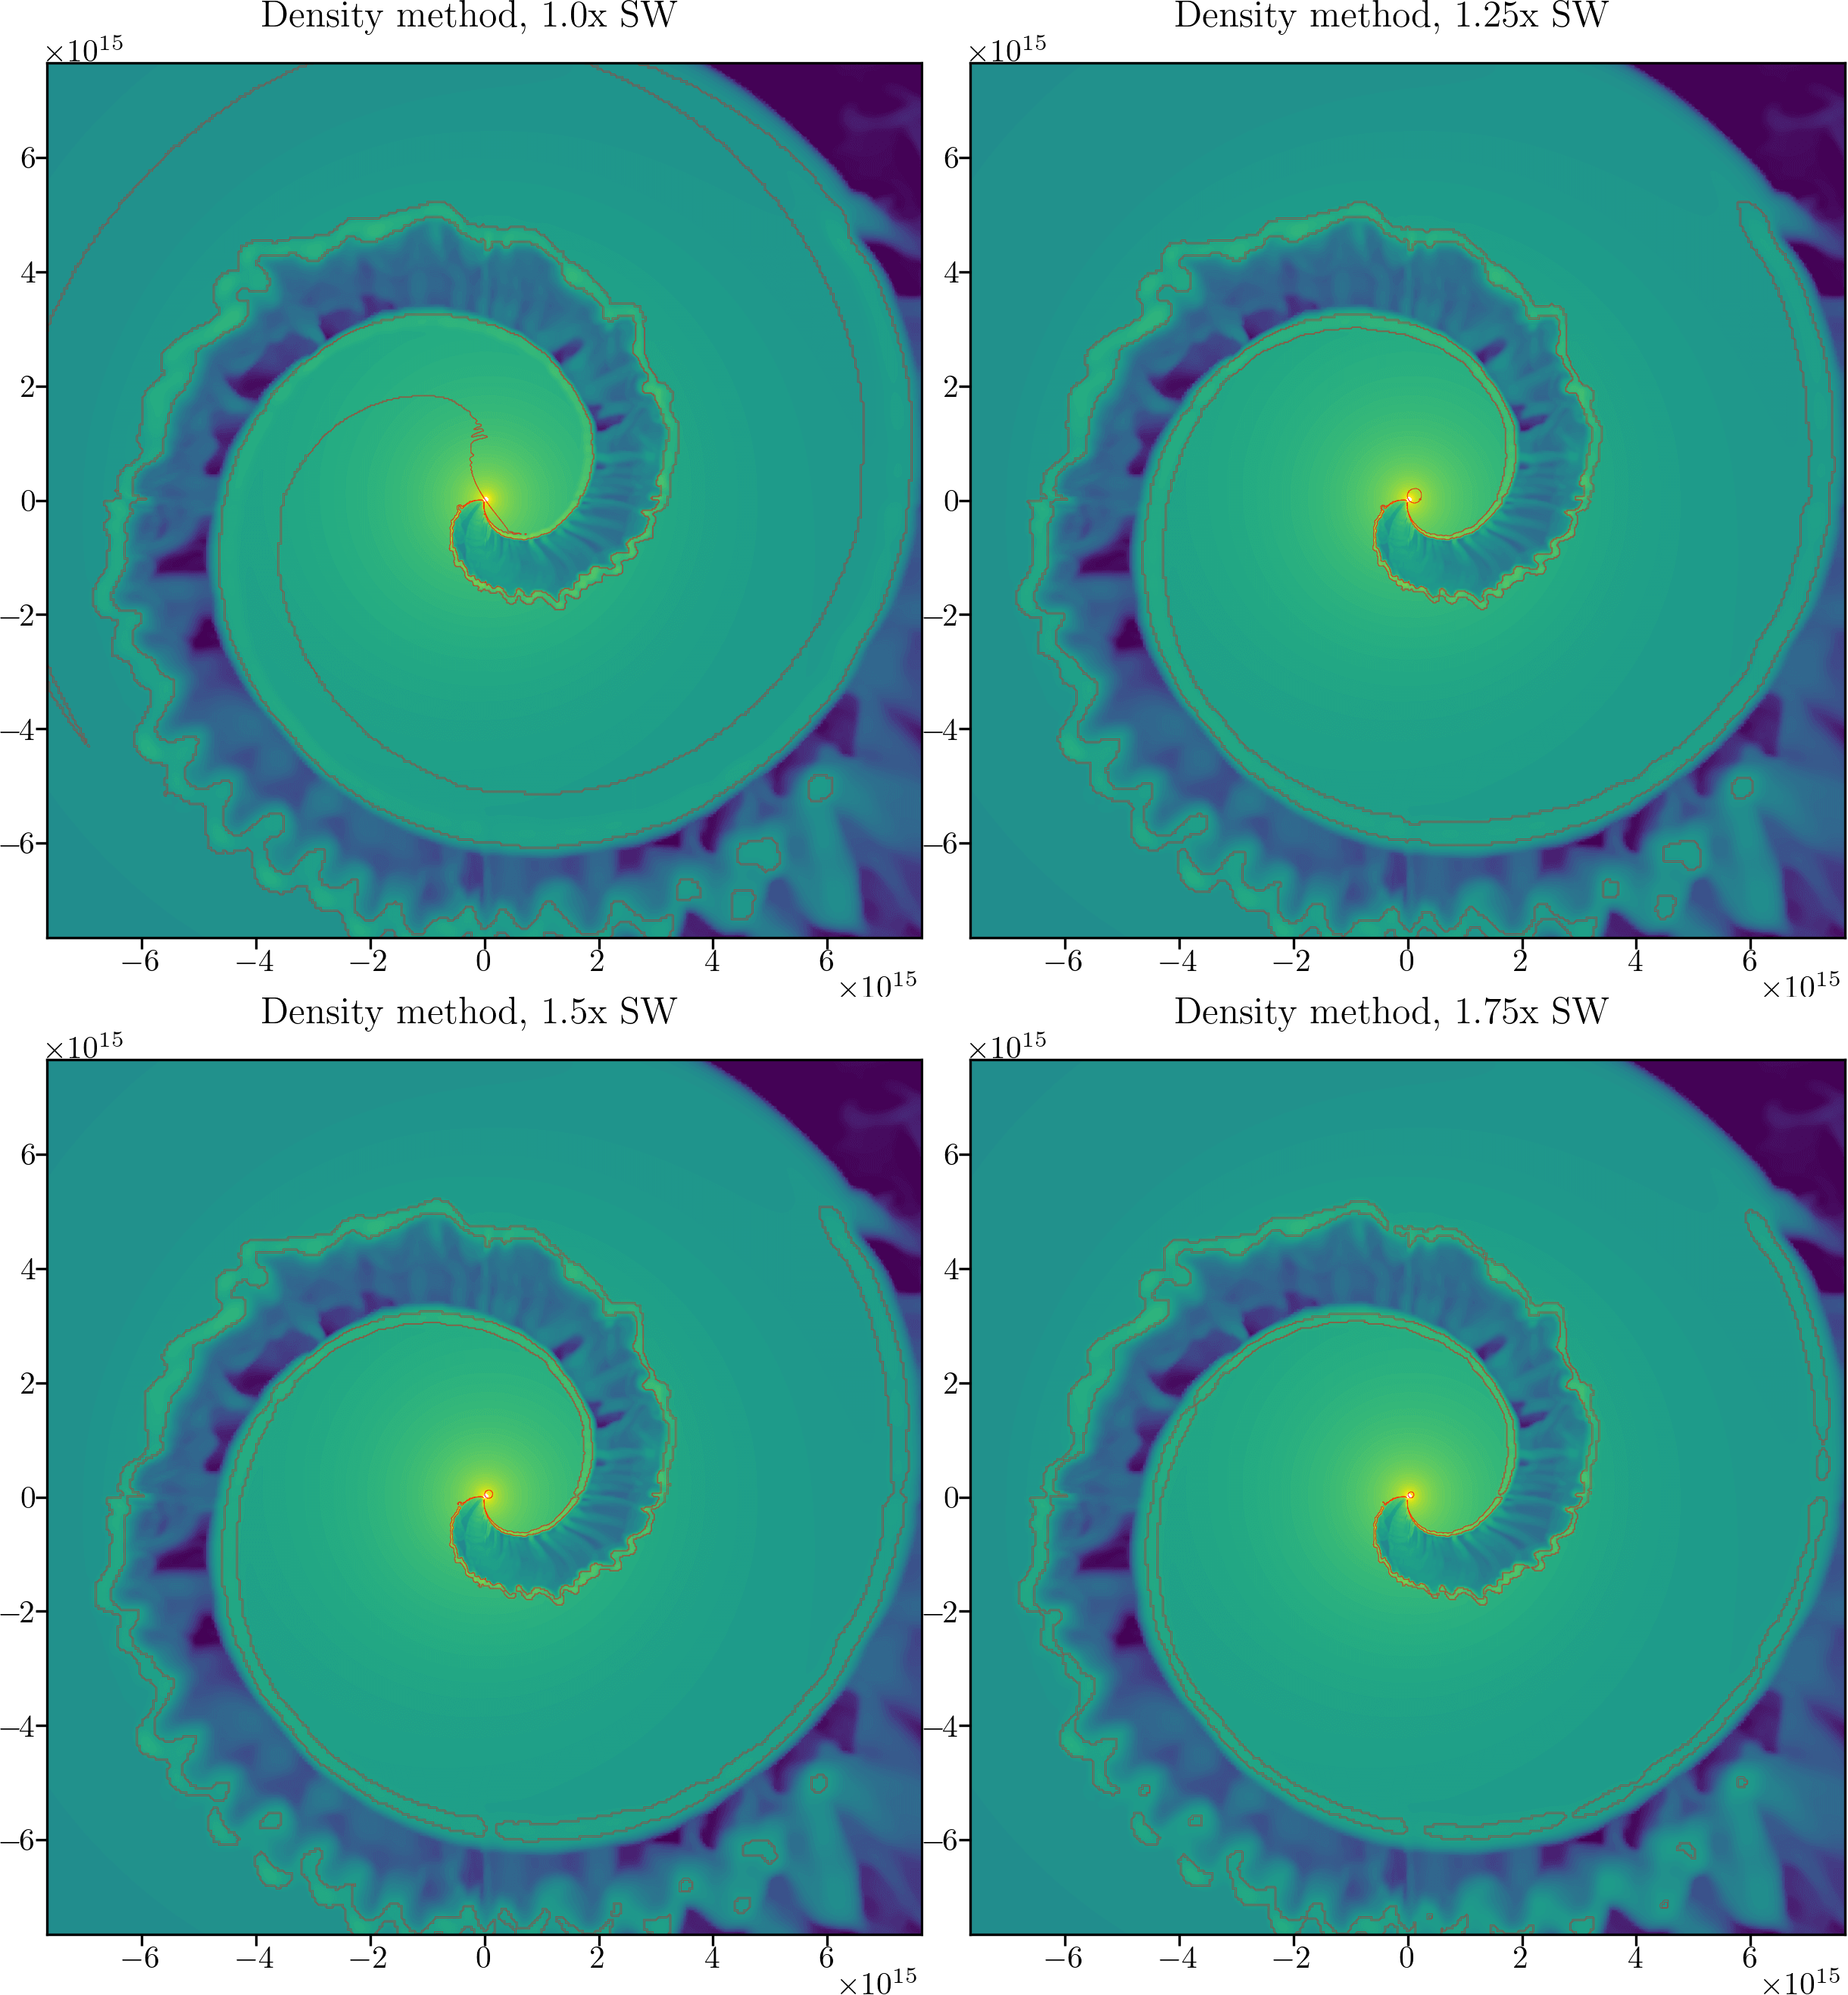
\includegraphics[width=5in]{assets/overdensity-method.png}
  \caption[Comparison of threshold values for over-density method]{Comparison of threshold values for the over-density method of determining if a cell resides in the wind collision region.
  A threshold value of $1.25\rho_\text{SW}$ was chosen as it most accurately determined if the cell was in the post-shock region.}
  \label{fig:overdensity-threshold}
\end{figure}

\section{Results}

\subsection{Radiative processes}

The first round of simulations were performed in order to assess whether the implemented cooling model would influence dust formation within the WCR.
This was found to be the case, figure \ref{fig:coolingprocess-dustproduction} shows that without cooling only a marginal amount of dust formation occurs, largely due to propagation of dust grains into the simulation, dust destruction also appear to be occurring, with the average grain radius radius reducing over the course of the simulation. 
Dust production for the radiative processes simulations is significantly higher, with the \texttt{fullcool} simulation appearing to have consistently higher dust formation rates than \texttt{plasmacool}.
This is sensible, as \ref{fig:postshockcoolcomparison} shows that at immediate post shock temperatures small dust grains present strongly influence immediate post-shock cooling, allowing the wind to reach temperatures low enough for dust formation faster than if only plasma cooling was considered.

\begin{figure}
  \centering
  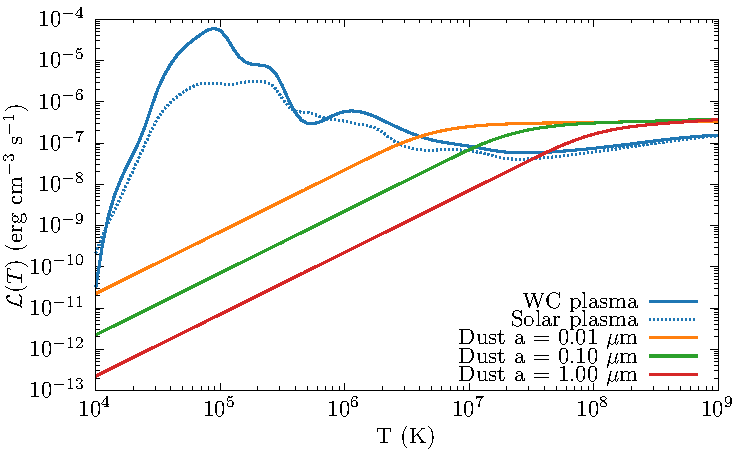
\includegraphics{assets/dust-plasma-cooling-comparison/cooling-comparison-forpaper2.pdf}
  \caption[Comparison of dust and plasma cooling rates in post-shock environment]{Comparison of plasma cooling to dust cooling with varying grain sizes in a typical post-shock flow, where $\rho_g = 10^{-16} \, \si{\gram\per\centi\metre\cubed}$ and a dust-to-gas mass ratio of $10^{-4}$.}
  \label{fig:postshockcoolcomparison}
\end{figure}

% 
In the case of the \texttt{fullcool} simulation, an average dust production rate of $\SI{5.4e-10}{\solarmass\per\year}$ is observed, with a peak formation rate of $\SI{7.1e-09}{\solarmass\per\year}$, this fluctuation appears to be due to dust forming mostly in high density instabilities (figure \ref{fig:coolingprocess-dustproduction}).
The fluctuations occur multiple times per orbit, but do not appear to be related to the orbital motion itself.

\begin{figure}
  \centering
  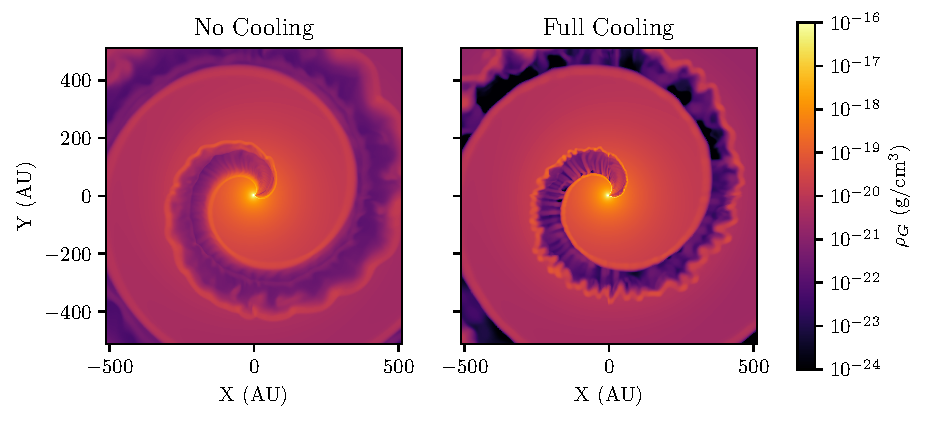
\includegraphics{assets/results/radiative/radiative-rho.pdf}
  \caption[Instabilities due to cooling]{Density comparison for \texttt{nocool} and \texttt{fullcool} models, with cooling enabled instabilities are far more prevalent, with pockets of very high density material within the WCR.}
\end{figure}

\begin{figure}
  \centering
  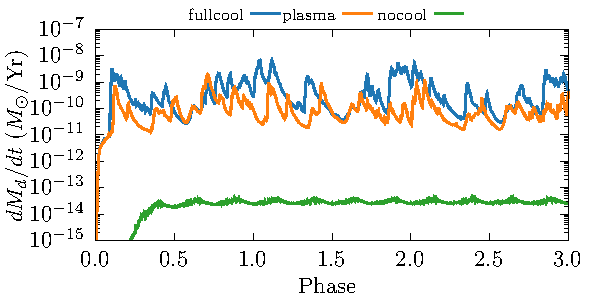
\includegraphics{assets/cool-results/cool-phase-dust_rate.pdf}
  \caption[Comparison of dust formation rates with cooling methods]{A comparison of dust formation rates as cooling mechanisms are changed. Without adequate cooling barely any dust is formed, while dust formation does increase with all cooling mechanisms enabled plasma cooling is still the dominant cooling process for dust production.}
  \label{fig:coolingprocess-dustproduction}
\end{figure}

% //TODO plot showing simulation a t 1.0, 2.0 and 3.0 phase, showing difference in dust formation

% Temperature and dust formation on leading edge

As cooling is significant in the post-shock WR wind, non-adiabatic compression is allowed to occur, resulting in much higher post-shock densities (figure \ref{fig:postshockcompression}).
Gas rapidly cools within this post-shock region, corresponding to where energy losses were stated to be important in \textcite{usov_stellar_1991}, this results in ideal conditions for dust formation, especially within the higher density instabilities.
A similar effect for the OB wind is not observed, as radiative energy losses are are not influential on the dynamics of the flow, due to the faster, significantly thinner stellar wind.
Figure \ref{fig:postshocktemperature} shows that the \texttt{fullcool} simulation has a similar immediate-post shock temperature to an adiabatic model, however this region cools within an extremely short timescale, allowing the nascent dust grains to grow.
Figure \ref{fig:full-radiative-z} shows dust clumps forming shortly after initial wind collision, 
after initial rapid formation rapid dust production tapers off as the post-shock wind becomes more diffuse. 
Temperature is also significantly more affected in the leading edge relative to the orbital motion, leading to a larger portion of dust forming in this region.

% It is believed that this effect is due to the region not being within line-of-sight of the WC star, and as such not being subject to the same degree of oblique shocks from the stellar wind.
% Actually it may be an idea to discuss this with Julian, since it could be a number of factors, maybe even orbital motion, or the wind colliding with late-WCR, leading to more compression better cooling? would explain instabilities
% Julian noted in his 2009 paper that a similar principle was observed
% Most likely due to oblique collision, between 
\textcite{pittard_3d_2009} notes that in the case of colliding winds with $\eta = 1$ the trailing edge of the WCR takes part in oblique shocks with the stellar winds, while the leading edge is shadowed by the upstream WCR from the colliding material.
This results in a trailing edge with strong instabilities and cool, high density clumps of post-shock wind, while the leading edge has a low density flow that is not dominated by instabilities.
% significant distance preventing oblique shocks
This does not appear to occur in these low-$\eta$ systems, as oblique shocks occur at a much greater distance, when the stellar wind is significantly less dense.
% Need to discuss this a bit with julian, see if my reasoning is sound
Instead, the leading edge of the WCR appears to be much thinner and denser than the trailing edge, this is believed to be due to the leading edge interacting with the outflowing material due to the systems orbital motion, sweeping up material and obliquely shocking the downstream WCR. % This needs further work, but I think thats a working theory
% Dust formation occurs some distance from the immediate post-shock region, time to cool, in agreement with observations, see williams 1990
% Formation appears to stagnate after this formation period, insufficient density due to diffusion?
Most dust formation occurs in the downstream post shock region, as soon as the post-shock wind has sufficiently cooled.
Furthermore dust formation slows significantly as the post-shock wind begins to diffuse, limiting overall dust formation to a region around 100 AU from the WCR apex. % This needs to be more stringent, no time for that right now
This is in agreement with the research by \textcite{williams_dust_1990} and \textcite{hendrix_pinwheels_2016}, which note that there is a limited region suitable for dust formation.
% Section needs a diagram showing the described contact surfaces, might be a good idea to name them, alpha beta contact surfaces? Use the eta graphs for baseline

\begin{figure}
  \centering
  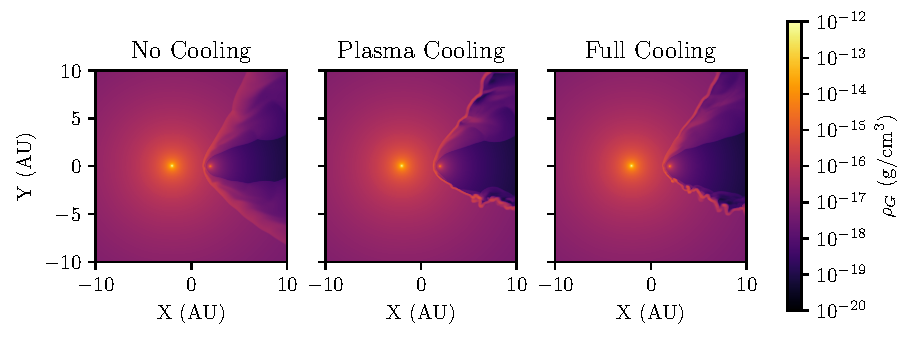
\includegraphics{assets/results/radiative/radiative-crop-2-rho.pdf}
  \caption[]{}
  \label{fig:postshockcompression}
\end{figure}

\begin{figure}
  \centering
  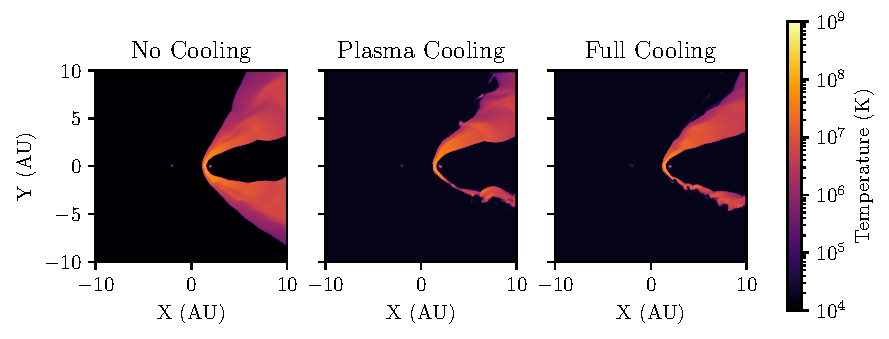
\includegraphics{assets/results/radiative/radiative-crop-2-temp.pdf}
  \caption[]{}
  \label{fig:postshocktemperature}
\end{figure}

\begin{figure}
  \centering
  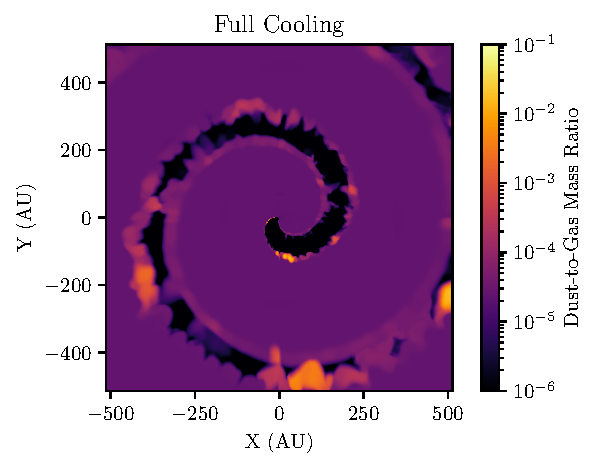
\includegraphics{assets/results/radiative/z.pdf}
  \caption[\texttt{Baseline} simulation $z$, full extent]{Full extent of \texttt{baseline} simulation, showing dust-to-gas mass ratio, dust typical forms in clumps within instabilities, leading to variation of dust formation as the simulation progresses.}
  \label{fig:full-radiative-z}
\end{figure}


% Orbital variation in general, simulation run out to a longer distance, no major variance between orbits

% \begin{figure}
%   \centering
%   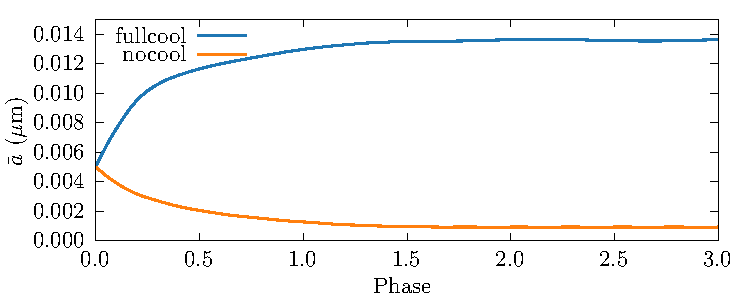
\includegraphics{assets/cool-results/cool-phase-avg_a.pdf}
%   \caption[Comparison of grain radii with varying cooling methods]{Average grain radius throughout simulations with varying cooling methods, plasma and dust are close to being the same, however without any cooling processes dust destruction is dominant, resulting in grain radius falling below the initial grain radius, $a_i$.}
%   \label{fig:coolingprocess-grainradius}
% \end{figure}

\subsection{Mass loss rate variation}

% High mass loss rate for both stars results in a high rate of dust formation 
Dust formation in the set of simulations which vary mass loss rate was found to be dependent on strong winds from either the WC or OB stars.
As can be seen in figure \ref{fig:mdotdustproductionrate}, the rates are stratified into similar dust production rates for simulations with similar values of $\eta$; simulations with an $\eta$ of 0.01 produce the most dust, while simulations with $\eta = 0.04$ producing approximately 3 orders of magnitude less dust than the most productive simulations.
% Note this is not related to the amount of wind, appears to be proportional to the wind momentum ratio instead 
However, the heightened dust production rate does not correspond to the summated mass loss rate of the system.
For instance, \texttt{mdot-1} and \texttt{mdot-3} produce on average $\sim 10^{-8}\,\si{\solarmass\per\year}$ with a net mass loss rate with factors of 1.99 and 1.01 higher than the baseline simulation respectively.
While the mass loss rate for each star varies throughout these simulations by a factor of 4, the dust production rate varies significantly more than that, further ruling out the increased rate of dust production being due to there simply being more mass in the simulation.
% Indicates that cooling is not the only factor, a strong shock must form first
All simulations in this system have comparatively low values for $\chi_{WR}$, which suggests that the simulations are at least weakly radiative, this implies that cooling is not the only governing factor, and that a strong shock must also form.

\begin{figure}
  \centering
  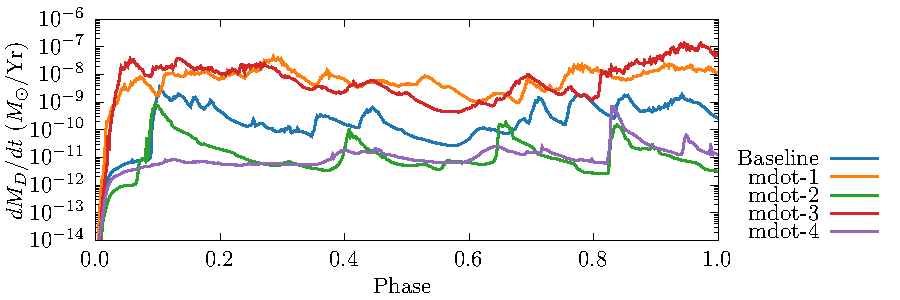
\includegraphics{assets/mdot-results/mass-loss-phase-dust_rate.pdf}
  \caption[Dust production rate for simulations varying mass loss rate]{A comparison of dust production rates for simulations that vary mass loss rate, $\dot M$, simulations with either a strong primary or secondary wind produce similar levels of dust, whilst if either wind is weaker, dust production rate is reduced.}
  \label{fig:mdotdustproductionrate}
\end{figure}

\subsection{Terminal velocity variation}
\label{sec:paper1vinfresults}

\begin{figure}
  \centering
  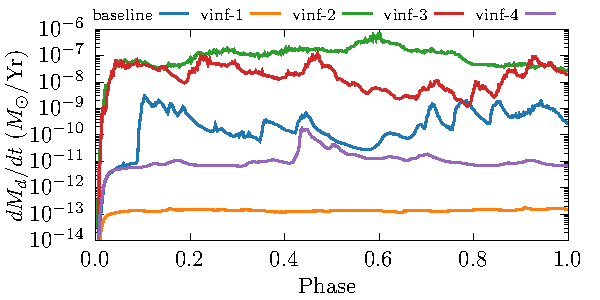
\includegraphics{assets/vinf-results/vinf-phase-dust_rate.pdf}
  \caption[]{Comparison of dust production rate for simulations varying wind terminal velocity, $v^\infty$. Simulations }
  \label{fig:vinfdustproduction}
\end{figure}

Varying wind terminal velocity appears to have an extremely strong effect on dust formation, with effects that are not solely related to $\eta$.
% Slow WR wind = strongly cooling high dust formation
Dust production rate is extremely high in the case of \texttt{vinf-2}, which has an extremely slow wind velocity of \SI{500}{\kilo\metre\per\second}, which is on the low end of expected wind terminal velocities for WR stars, and has a wind velocity closer to that on a typical LBV star.
This very slow, dense wind is highly influenced by radiative cooling in the post-shock environment, driving thermal instabilities, leading to high density pockets of cooled gas, ideal for dust formation.
% Observation shows extremely instability influenced winds, discuss instabilities in general, Kelvin Helmholtz?
This can be seen in figure \ref{fig:vinfrhodcomp}, where \texttt{vinf-2} produces large quantities of dust in the WC-stagnation point interaction region, 
% Shock temperature much lower
The initial shock temperature for \texttt{vinf-2} was also significantly lower than 
% Note increased dust in non-shocked wind, this was found to be a fraction of the overall dust produced
It should be noted that dust production in general increases outside of the WCR, this is largely due to significantly higher wind density within the WC wind.
This is due to the model not currently featuring destruction due to photodissociation, which can be included in future models.
Despite this, the dust production outside of the WCR does not significantly impact the total dust production rate, and numerical analysis of dust production such as in figure \ref{fig:dsepdustproduction} does not include dust produced outside of the wind collision region.
%//TODO find actual value
In the case of a fast WC wind however, dust production effectively ceases,  with an average dust production rate of $\SI{8.9e-13}{\solarmass\per\year}$, multiple orders of magnitude less than \texttt{vinf-4}, which has a similar wind momentum ratio.

% Fast OB wind = very strong shock

% \begin{figure}
%   \centering
%   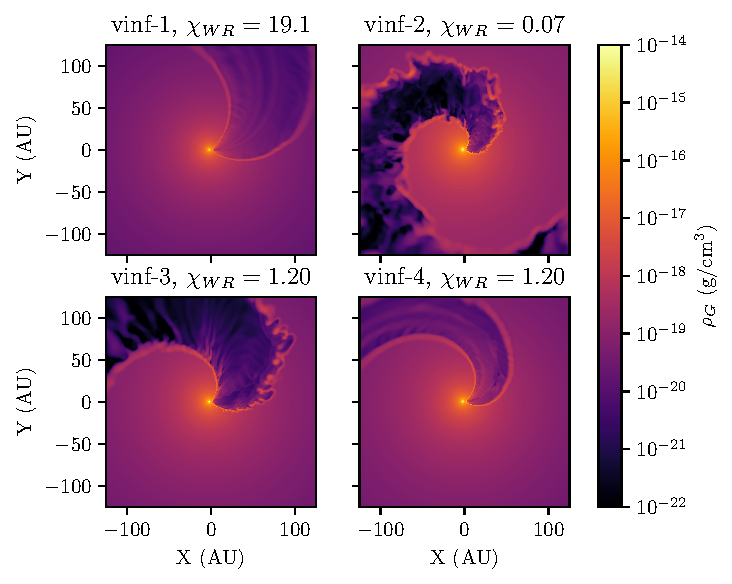
\includegraphics{assets/results/vinf/vinf-finished-rho.pdf}
%   \caption[]{Comparison of terminal velocity variation simulations, simulations with a high ratio of wind velocities appear to exhibit instabilities leading to strong wind mixing, as these seem to be based on velocity shear, it is reasonable to assume that the structure of the WCR is dominated by Kelvin-Helmholtz instabilities.}
%   \label{fig:vinfdensitycomp}
% \end{figure}

\begin{figure}
  \centering
  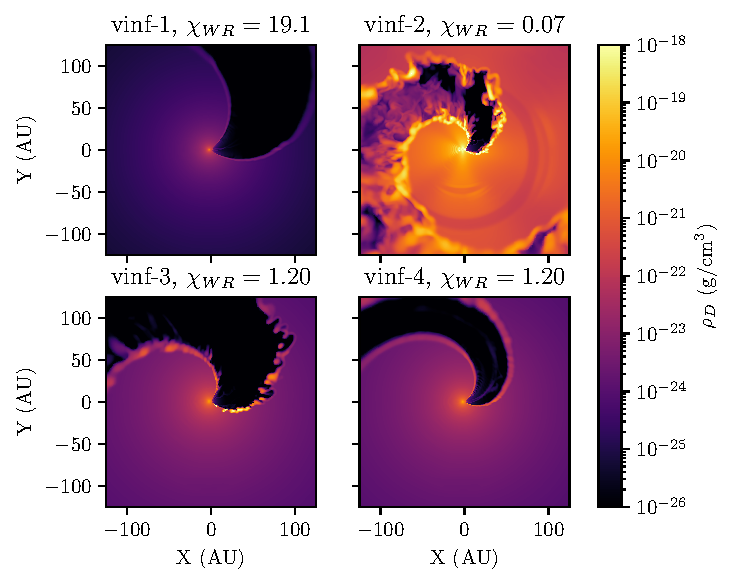
\includegraphics{assets/results/vinf/vinf-finished-rhod.pdf}
  \caption[Dust density comparison of terminal velocity varying systems]{Comparison of dust density in $v^\infty$ variation simulations, simulations with either a low OB wind velocity or high WC wind velocity produce large quantities of dust. Simulation \texttt{vinf-1}, which has a high velocity WC wind, does not produce any appreciable dust within the WCR.}
  \label{fig:vinfrhodcomp}
\end{figure}

% Focus on vinf-3 and vinf-4 figure analysis, zoom out, VINF3 has a very stable secondary wind but much stronger instabilities, implies uncertainties due to velocity differential as well? More dust produced even though mean temperature of this simulation is much higher, implies cooling not the only mechanism, strong shock + additional isntabilities
Simulations \texttt{vinf-3} and \texttt{vinf-4} are of note as when the secondary wind velocity was altered, drastic changes to the dust formation rate occur, similar to modifying the mass loss rate of the secondary star as detailed in the previous section.
% Instabilities in secondary wind can 
Instabilities due to the secondary wind appear to be the result of this, a greater secondary wind velocity would lead to a greater velocity shear along the discontinuity, resulting in Kelvin-Helmholtz instabilities.
Both \texttt{vinf-2} and \texttt{vinf-3} exhibit this behaviour, and both have a terminal velocity ratio, $\frac{v_\text{OB}^\infty}{v_\text{WR}^\infty} = 4$.
This would augment the already present thermal instabilities due to radiative cooling, leading to a less ordered, clumpy post-shock environment \parencite{stevens_colliding_1992}.
This is found to be the case with \texttt{vinf-3}, which has a far greater amount of dust formation within the WCR, and has a significantly more mixed wind.
This can be seen in figure \ref{fig:obvinfzcomp} where \texttt{vinf-3} and \texttt{vinf-4} are directly compared, despite both simulations having an adiabatic second wind, the presence of a much faster secondary wind results in a velocity shear that produces a much broader WCR, with high density pockets formed within instabilities, which appear to produce the bulk of dust. 
This suggests that prolific dust formation occurs in  a post-shock primary wind shaped by instabilities, produced either from strong radiative cooling, or through a strong velocity shear, leading to K-H instabilities.
Radiative cooling is also important beyond thermal instabilities, in order to reduce to adequate temperatures in the high-density immediate post shock flow.
% Stratification of simulations does not occur in the same way, 
Results appear to be stratified somewhat in terms of $\eta$, where simulations where $\eta = 0.04$ produce significantly more dust than simulations with more imbalanced winds.
However, this dependence is different to the mass loss rate simulation subset, and the stratification is less apparent, this suggests a loose correlation between $\dot M_D$ and $\eta$ when $v_\infty$ is varied.
% Direct eta correlation, however fast drop of dust formation for Fast WR wind model


% //TODO add LBV to mass loss rate chart


% Starting to form concept that chi is also not fundamental, cooling not everything, formation of strong instabilities however by any mean is most important


% Purpose of radiative line driving, close binaries may have lower OB wind velocity, leading to less dust formation
% Refer to radiative inhibition 
% Cannot be simulated with current version of code, but interesting to consider

\begin{figure}
  \centering
  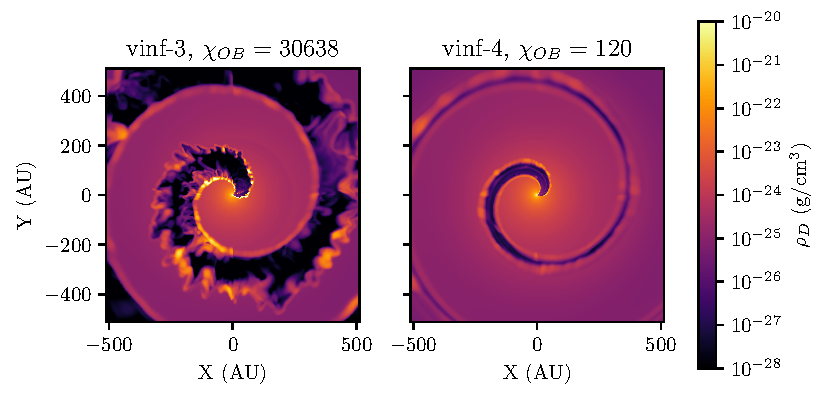
\includegraphics{assets/results/vinf/vinf-rhod.pdf}
  \caption[OB terminal velocity wind dust comparison]{Comparison of dust density in simulations with at modified OB wind terminal velocities, simulations are fully advected with $\phi = 3.0$, dust formation and instabilities are far more pronounced in \texttt{vinf-3}, which has wind velocity a factor of 4 larger than \texttt{vinf-4}.}
  \label{fig:obvinfzcomp}
\end{figure}

\begin{figure}
  \centering
  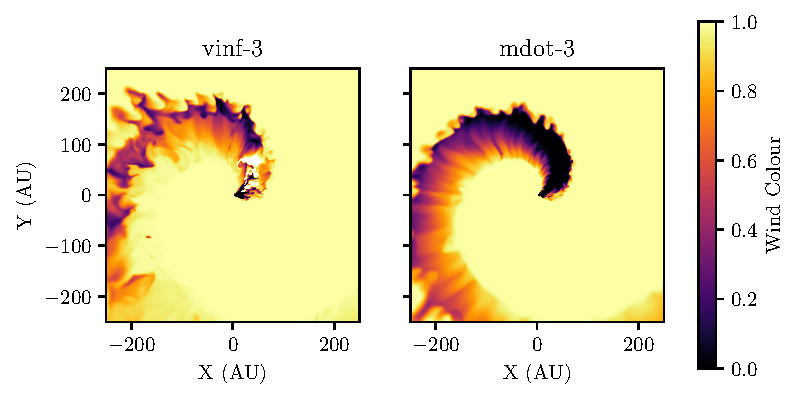
\includegraphics{assets/results/mixed/eta-004-comparison-r0.pdf}
  \caption[Wind colour comparison of $\eta = 0.04$ winds]{Comparison of wind colour in simulations \texttt{vinf-3} and \texttt{mdot-3}, wind mixing is significantly more pronounced, with a pronounced post-shock WR wind that appears to be strongly influenced by Kelvin-Helmholtz instabilities, due to the increased wind velocity imbalance and lower degree of cooling.}
  \label{fig:eta004comparisoncolour}
\end{figure}

\begin{figure}
  \centering
  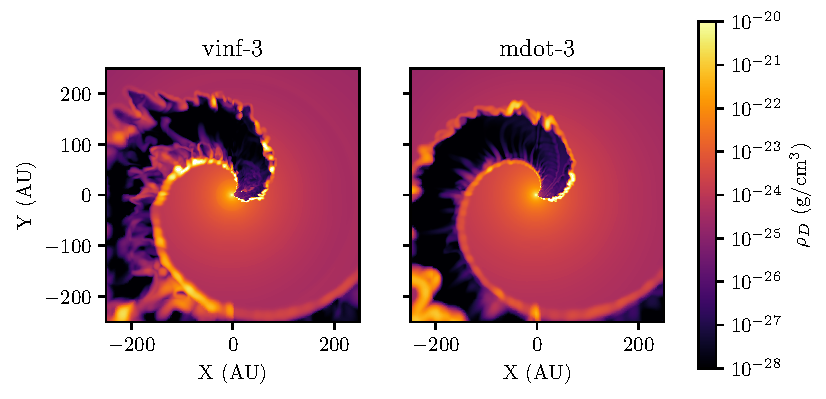
\includegraphics{assets/results/mixed/eta-004-comparison-rhod.pdf}
  \caption[]{Comparison of dust density in simulations with a strong secondary wind, \texttt{vinf-3} \& \texttt{mdot-3}, dust in \texttt{vinf-3} is produced to a much higher degree in the trailing edge of the wind, and increased mixing of the wind due to Kelvin-Helmholtz instabilities has led to dust forming throughout the WCR, rather than at the WC-stagnation point boundary.}
  \label{fig:eta004comparisonrhod}
\end{figure}

By directly comparing two prolific dust producing models with $\eta = 0.04$, \texttt{vinf-3} and \texttt{mdot-3}, we can see that both WCRs are dominated by instabilities.
\texttt{vinf-3} in particular appears to be much more thoroughly mixed (figure \ref{fig:eta004comparisoncolour}), with a much larger trailing edge that produces large quantities of dust (figures \ref{fig:eta004comparisonrhod}).
This additional degree of instability appears to be due to Kelvin-Helmholtz instabilities, which grow significantly as the post-shock gas flows away from the stagnation point, as described in \textcite{stevens_colliding_1992}.
These simulations produce approximately the same amount of dust, with \texttt{vinf-3} also consistently producing dust in the trailing edge of the WCR.
From these results it is clear that a high dust production rate is dependent on a highly imbalanced wind, with a slow WC and fast OB wind, as this drives a strong shock, leading to strong cooling and thin-shell instabilities, while also producing additional high density regions and mixing through Kelvin-Helmholtz instabilities.

% \begin{figure}
%   \centering
%   \includegraphics{assets/vinf-results/vinf-phase-avg_a.pdf}
% \end{figure}

% //TODO include table of average/peak dust formation rates for simulations with vinf and mdot variation

\subsection{Separation variation}

% Direct chi correlation, could also be due to weaker shocks

As can be seen in figure \ref{fig:dsepdustproduction} there is a clear correlation between separation distance and dust formation rate, with dust production drastically increasing as orbital separation is decreased.
This influence on the dust formation rate is non-linear, with a doubling of the separation distance increasing the dust production rate by approximately one order of magnitude.
Variation of the dust production rate also appears to increase as separation distance is reduced, leading to instances where a simulation may temporarily produce more dust than a simulation with a tighter orbit, such as the case with \texttt{dsep-4AU} and \texttt{dsep-8AU} at $\Phi = 0.6-0.7$.
some of this could be related to numerical error, however, it is clear that systems with closer orbits are far more instability driven, as can be seen in figure \ref{fig:dsepinstabilities}.
As we have previously discussed, instabilities drive slightly intermittent, but highly effective dust formation, which can be seen in the clumpy dust formation of \texttt{dsep-4AU} and \texttt{dsep-8AU} in particular.

% Discuss radiative line driving model
It would be interesting to consider how 

due to radiative stagnation and braking from the 

Unfortunately, the current model does not simulate this effect, instead relying on a terminal velocity wind model. This would be an interesting avenue of research, however.

%//FIXME this needs work! 32AU result is instead labelled as 64AU and zooms aren't consistent!

\begin{figure}
  \centering
  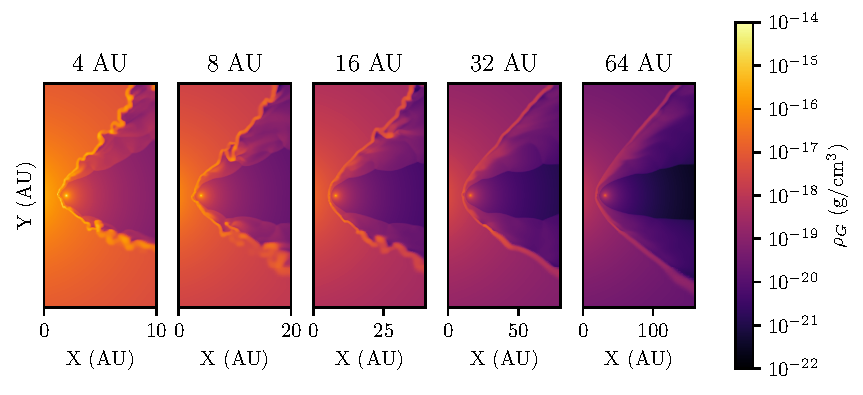
\includegraphics{assets/adiabatic-flow/instab-comp-rho.pdf}
  \caption[]{A comparison of the structures of simulations varying $d_\text{sep}$, the scale of each plot has been changed to allow for a similar feature size, as can be seen simulations with a closer separation distance have collision regions whose structure is more strongly influenced by instabilities, particularly thin-shell instabilities brought on by the presence of radiative cooling within the WCR.}
  \label{fig:dsepinstabilities}
\end{figure}

% Dust yields

\begin{figure}
  \centering
  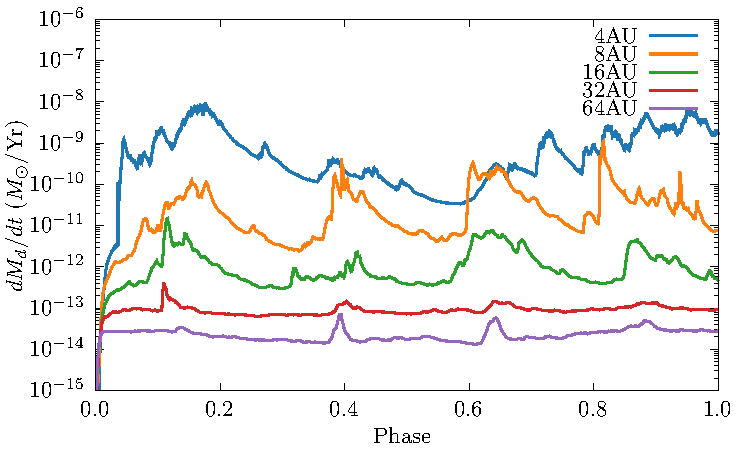
\includegraphics{assets/dsep-results/dsep-phase-dust_rate.pdf}
  \caption[Dust formation rate vs. binary separation distance]{A comparison of dust formation rates versus orbital phase for a set of simulations that vary separation distance, $d_\text{sep}$. A clear inverse relationship between separation distance and dust production rate exists, most likely due to the stellar winds becoming more diffuse further from their origin stars, leading to weaker shocks and a WCR that behaves more adiabatically.}
  \label{fig:dsepdustproduction}
\end{figure}

A clear trend with orbital separation is that dust formation increases drastically as the stars are positioned closer together, at high degrees of separation dust formation ceases, and average grain size drops below the initial value of $50 \text \AA$.

The bulk of dust growth occurs in the immediate post shock region, as dust is rapidly cooled and at a high enough density for dust formation to occur.

This matches observations of episodic dust forming systems, where infrared emission due to dust is maximised at or shortly after periastron passage. This also lends further evidence that dust formation rates are not influenced solely by the momentum ratio, as this is kept constant, and instead is strongly influenced by the wind density at collision and post-shock cooling. 

% Some periodicity, shared between stars are various phases, this could be due to spirals formed as the stars rotate? Pinwheel structure?

% Include table of formation rates for orbital separation

\section{Conclusions}

% General links of 


\subsection{Dust formation sensitivity}

% Dust formation appears to be extremely sensitive to initial conditions, particularly terminal velocity
The simulations in this paper were conducted over a fairly limited range of initial conditions for mass loss rate and wind terminal velocity, wind velocity and mass loss rates are varied by no more than a factor of 4.
Despite this, dust production varies by up to 6 orders of magnitude, in the case of wind terminal velocity.
This suggests that dust formation is extremely sensitive to the initial conditions of 
Dust formation rate also varies in accordance with the separation distance, but is somewhat less sensitive to change, this would present itself more in terms of WCd systems that exhibit periodic dust formation, as WC stars do not undergo significant variability of their wind properties over the timescale observed in periodic WCd systems.
% Highly speculative, bring this one down to earth
This would present an interesting factor in the case of CWB systems with an LBV partner such as $\eta$ Carinae, as an LBV would result in a highly variable wind collision region outside of fluctuations due to separation distance \parencite{nazeChangingWindCollision2018}.
% Briefly discuss extrapolation of results, other systems
The baseline system, WR98a, has a significantly lower mass loss rate than other well-characterised WCd systems, such as WR140 and WR04, the WC star in WR 140 has a mass loss rate an order of magnitude larger than WR98a, for instance.
% Allude to additional research, covered in papers 2 and 3?
As such, future research in this topic will cover these systems, as an exploration of more extreme conditions would be conducive to demonstrating the veracity of this dust model.
% What does that even mean buddy

\subsection{Radiative inhibition and its influence on eccentric WCd systems}

% Purpose of radiative line driving, close binaries may have lower OB wind velocity, leading to less dust formation
% Refer to radiative inhibition 
% Cannot be simulated with current version of code, but interesting to consider

The lack of radiative line driving, and instead using a terminal velocity model for stellar winds is an important consideration when assessing the results of this paper.
It has been established over the course of this paper that dust production rate is highly dependent on the wind velocity of either stars stellar wind; hence any mechanism that influences the wind velocity over the course of an orbit can be a potential mechanism for the variable dust formation in CWB systems with high eccentricities.
Whilst orbital separation is a definite factor in changing dust formation rates, with tightly bound orbits producing the most dust, it can be argued that as stellar separation decreases as the stars approach periastron, dust production will increase, and taper off as the star moves beyond this point as it heads towards apastron.
This can be seen in observations, as dust production reaches its peak at periastron passage, however, dust formation ramps up extremely rapidly, whilst taking much longer to reduce \parencite{williamsDustFormationCollidingwind2008,williams_orbitally_2009}.
This asymmetry implies processes that occur more strongly as the system heads towards periastron than away from it.
Changes to wind velocity may prove to be a source of mechanisms behind this effect.

As the wind is highly imbalanced, the velocity of the OB stellar wind will be lower than the expected terminal velocity due to insufficient acceleration before the wind undergoes radiative inhibition and braking.
Whilst dust formation benefits from a slow primary wind, a slow secondary wind can drastically reduce the rate of dust formation.
For instance, in the case of WR 140 at periastron passage, the O4-5 companion star with a terminal wind velocity of $\SI{3200}{\kilo\metre\per\second}$ was found to have a line-driven wind velocity $\sim 84\%$ of $v^\infty$ before collision with the WCR at $r_{OB}$ (figure \ref{fig:wr140-stagnation-obwind}).
As demonstrated in the velocity variation simulations, halving the wind terminal velocity can reduce the dust formation rate by approximately 2 orders of magnitude, due to a weaker wind collision shock and a reduction in instabilities.
A reduction of $84\%$ in the secondary wind velocity with no corresponding reduction in the primary wind velocity would result in a noticeably lower overall dust production rate for a brief period, and may be a potential factor for the rapid onset and slow decline of dust production after periastron passage. %Why?
% It would be a good idea to run some simulations in paper 3 at WR140 periastron with radiative line driving estimates, might be an interesting avenue of research
% Mention orbital velocity at periastron passage, for certain systems this can be very high, relative velocity of winds increased by factor of ~1.2 for WR 140, this would explain attack/decay pattern 

\begin{figure}
  \centering
  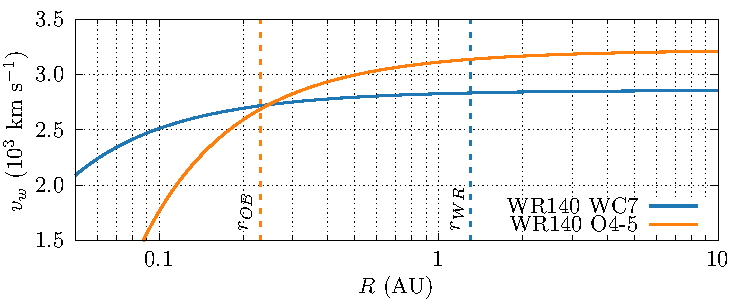
\includegraphics{assets/stagnation-point/stag.pdf}
  \caption[Stagnation point wind velocity]{Graph of secondary wind velocity and density as a function of distance from the stellar surface due to radiative line driving for the WR 140 system, as well as an estimation of $r_{OB}$ and $r_{WR}$ at periastron passage. While at periastron the WC7 wind is travelling at approximately terminal velocity, the O4-5 companions wind is travelling at $\sim 84\%$ of terminal velocity before coming into contact with the WCR. CAK parameters were estimated to be $k = 0.37$, $\alpha = 0.60$ for the O4-5 star and $k=0.48$, $\alpha = 0.57$ for the WC7 star.}
  \label{fig:wr140-stagnation-obwind}
\end{figure}

\subsection{Wind mixing within the WCR}

%This may need additional work, and is largely speculation 

While interaction between Hydrogen and dust grains is not simulated by the dust model, \textcite{leteuffModelDustFormation2002} notes that Hydrogen could be a potential catalyst for amorphous carbon grain formation.
Figure \ref{fig:radiative-windmixing} shows that the wind is far more effectively mixed by instabilities if it is sufficiently radiative, an improved dust model which can calculate grain yields from chemical reactions could be used to investigate this further.
Implementation of a chemical model into Athena++ through passive scalar is a stated goal of Athena++, though it is still in development.
Additionally, a multi-wind model could be used to model the dynamics of grains, as larger grains carry significantly more than atoms in the stellar wind, and may not be necessarily co-moving in a turbulent wind environment.
% Improvements to model, multi-wind model, astrochemical model? Extremely large bounds for future work
% Mention single wind WC grain formation
It should also be noted that dust formation around single WC stars has been observed, suggesting that nascent grains are formed within the WC wind, and carried into the Colliding Wind Binary as implied by this dust model.

\begin{figure}
  \centering
  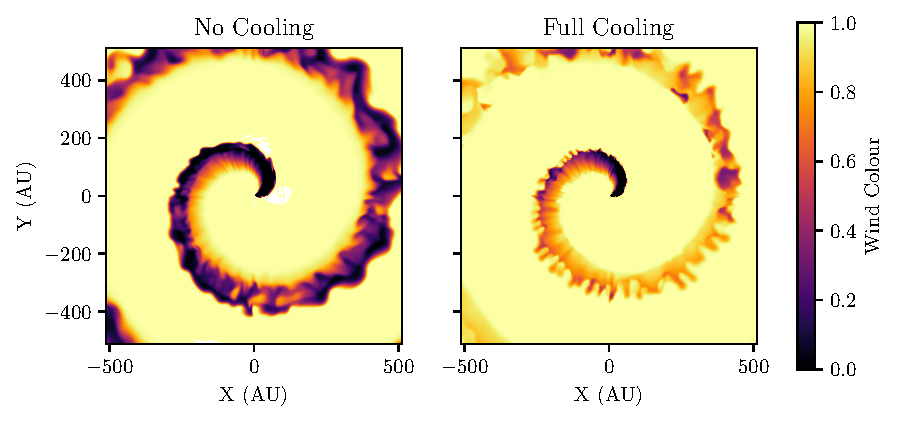
\includegraphics{assets/results/radiative/radiative-r0.pdf}
  \caption[Wind mixing due to radiative methods]{Wind ``colour'' for \texttt{nocool} and \texttt{fullcool} models, the WCR is more thoroughly mixed if the simulation is allowed to cool.}
  \label{fig:radiative-windmixing}
\end{figure}

\section{Summary and Conclusions}

The introduction of an advected scalar dust model into a numerical simulation

Whilst the current feature set is limited by the available remaining time in this project, future work in this vein can introduce additional dust formation

Another interesting avenue of research is the 